\chapter{Specification Theory}\label{ch:spec_theory}

\section{Quotient}
One of the essential operators in specification theory is Quotienting. This operator factors out the behavior from a larger component. It is required that for larger component, dividend $A_t$ and the smaller component, divisor  $A_s$ the relation on actions sets must hold: $\Sigma_i^S \subseteq \Sigma_i^T$ and $\Sigma_o^S \subseteq \Sigma_o^T$. As long as, these requirements are met, then the quotient of $A_t$ by $A_s$, which is denoted  $A_t$\textbackslash\textbackslash$A_s$ is the TIOA given by:
\begin{itemize}
	\item $Loc = Loc_T \times Loc_S \cup \{l_u, l_{\slashzero}\}$.
	\item $q_0 = (q_0^T,\ q_0^S)$.
	\item $Clk = Clk_T \uplus Clk_S \uplus \{x_{new}\}$.
	\item $Inv((q_T,\ q_S)) = Inv(l_u) = true$ and $l_{\slashzero} = \{x_{new}\leq 0\}$.
\end{itemize}
New state $l_u$ is universal state and state $l_{\slashzero}$ is inconsistent. The set of actions $Act = Act_i \uplus Act_o$ is given by $Act_i = Act_i^T \cup Act_o^S \cup \{i_{new}\}$ and $Act_o = Act_o^T$\textbackslash$Act_o^S$. The set of edges $E$ is defined by:
	
\begin{enumerate}
	\item if $q_T\in Loc_T, q_S\in Loc_S, a\in Act$ then $((q_T,q_S), a, \neg Inv_S(q_S), \{x_{new}\}, l_u)\in E$.
		
	This rule creates a new transition, which leads to the universal state with a guard that equals the original invariant of the existing inner specification.
	\item if $q_T\in Loc_T, q_S\in Loc_S$ then $((q_T,q_S),i_{new}, \neg Inv_T(q_T) \land Inv_S(q_S), \{x_{new}\}, l_{\slashzero})\in E$
		
	This rule is for the case, when the invariant of $A_T$ is not satisfied, while $A_S$ invariant is.
	\item if $(q_T, a, \varphi_T, c_T, q'_T)\in E_T$ and $(q_S, a, \varphi_S, c_S, q'_S)\in E_S$ this gives $((q_T,q_S), a, \varphi_T \land \varphi_S, c_T \cup c_S, (q'_T,q'_S))\in E$
		
	This rule takes care of all regular synchronization, where the guards of each component is satisfied.
	\item for each $(q_S, a, \varphi_S, c_S, q'_S)\in E_S$ with $a \in Act_o^S$ this give rise to $((q_T,q_S), a, \varphi_S \land \neg G_T, \{x_{new}\}, l_{\slashzero})$ where $G_T = \bigvee \{\varphi_T |(q_T, a, \varphi_T, c_T, q'_T)\}$.
		
	This rule handles the case, when in the outer component $A_T$ the matching guards are not allowing the inner component to generate output.
	\item if $(q_T, a, \varphi_T, c_T, q'_T)\in E_T$, $a\notin Act_S$ then $((q_T,q_S), a, \varphi_T, c_T, (q'_T,q_S))\in E$
		
	This rule handles the cases, where given $A_S$ action set, $A_T$ tries to take action, which is not within that set.
	\item for each $(q_T, a, \varphi_T, c_T, q'_T)\in E_T$ with $a \in Act_o^S$ this give rise to $((q_T,q_S), a, \neg G_S, \{\}, l_u)$ where $G_S = \bigvee \{\varphi_S |(q_S, a, \varphi_S, c_S, q'_S)\}$. 
		
	This rule takes care of all the cases, where $A_T$ takes an action, which is not allowed by any of the matching guards in $A_S$ thus leading to the universal state. 
	\item for each $a \in Act_i$ this gives rise to $(l_{\slashzero}, a, x_{new} = 0,\{\}, l_{\slashzero})$
		
	This rule makes $l_{\slashzero}$ state inconsistent
	\item for each $a \in Act$ this gives rise to $(l_u, a, true,\{\}, l_u)$
		
	This rule ensures, that the universal state has all possible behavior
\end{enumerate}

Figure \ref{fig:quotient} provides illustration of one step in the computation of a quotient. Quotients input set, $Act_i$, has the inputs to the outer component $A_T$ and the outputs of the existing inner component $A_S$ as well as a new fresh input action $i_{new}$, Figure \ref{fig:quotient} c. Output set $Act_o$ is the output set of bigger component in this case $A_T$, excluding the outputs handled by the smaller component $A_S$. Quotient provides with two new special states, $l_u$ universal state as well as $l_{\slashzero}$ inconsistent state. State $l_u$ serves all the cases, where the smaller component $A_S$ violates the guarantees of bigger component $A_T$, which implies quotient having no restrictions for the future behavior. State $l_{\slashzero}$, serves the purpose of cases, where the quotient would violate the assumptions of other components, by taking this action, \textcite{10.1007/978-3-642-17071-3_15}.

\begin{figure}
  \centering
  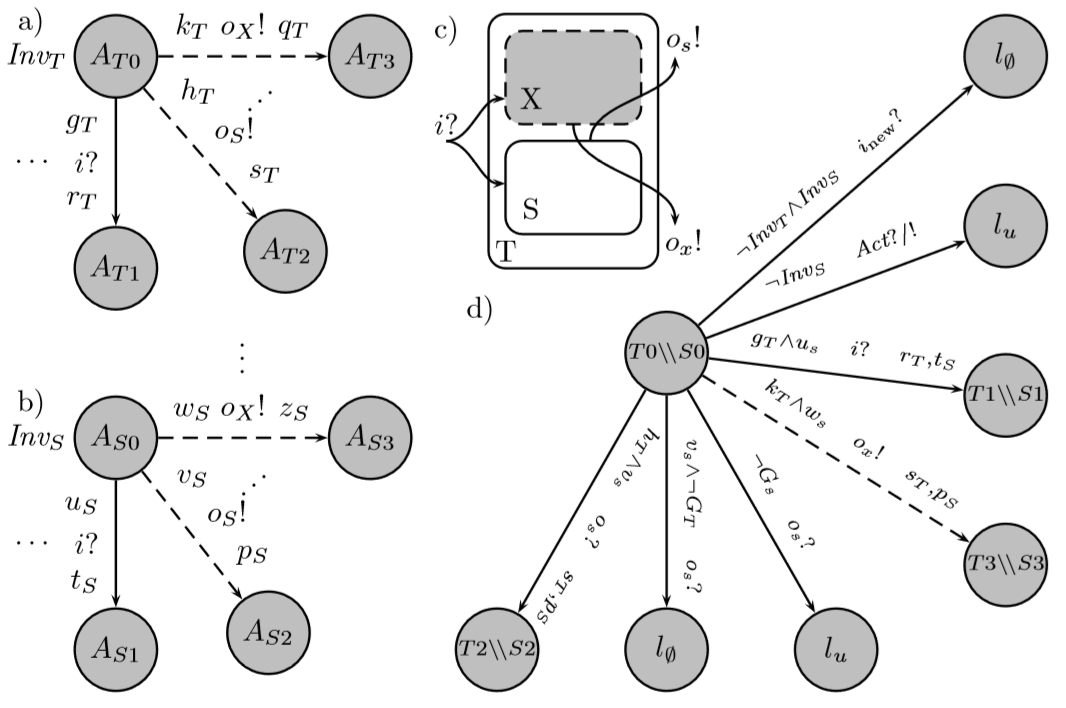
\includegraphics[scale=0.4]{figures/Quotient.png}
  \caption{Initial states of two TIOA a) $A_T$ b) $A_S$ c) communication flow d) resulting Quotient initial state \textcite{10.1007/978-3-642-17071-3_15}}
  \label{fig:quotient}
\end{figure}